\documentclass[landscape,a0]{article}
\usepackage{graphicx}
\DeclareGraphicsExtensions{.pdf,.png,.jpg}% No es necesario
\usepackage{wrapfig} %Figuras al lado de texto
%\usepackage[rflt]{floatflt} %
% indicar extensión.
\usepackage{amsmath,amssymb,amsfonts,latexsym,stmaryrd,caption,pstricks}
\usepackage[latin1]{inputenc}
\usepackage{pslatex}
\usepackage{bm}
\newtheorem{teo}{Teorema}
\newcommand{\R}{\mathbb{R}}
\newcommand{\Z}{\mathbb{Z}}
\newcommand{\Q}{\mathbb{Q}}
\newcommand{\C}{\mathbb{C}}
\newcommand{\N}{\mathbb{N}}
\newcommand{\I}{\mathbb{I}}
\newcommand{\F}{\mathbb{F}}
\newcommand{\gfrac}[2]{\displaystyle{\frac{#1}{#2}}}
\newcommand{\limite}[2]{\lim_{#1 \rightarrow #2}}
\newcommand{\ds}{\displaystyle}
\newcommand{\sen}{\mathop{\rm sen}\nolimits}
\newcommand{\senh}{\mathop{\rm senh}\nolimits}
\newcommand{\arcsen}{\mathop{\rm arcsen}\nolimits}
\newcommand{\arcsec}{\mathop{\rm arcsec}\nolimits}
%-----------------------------------------------------------------------


\begin{document} % Compilar PDFLaTeX
\begin{minipage}[b]{0.5\linewidth}
	% En el pre�mbulo:
	%\newtheorem{teo}{Teorema} est� en el pre�mbulo
	\begin{teo}[Teorema del valor Medio]\label{tvm}
		Sea $f(x)$ continua en $[a,b]$ y derivable en $]a,b[,$
		entonces $\exists\,\xi \in\,]a,b[$ tal que
		$$f(a)-f(b)= f'({\red\xi})(b-a)$$.
	\end{teo}
	En particular, siendo $f(x)=6-(x-2)^3+x$,
	$a=2$ y $b=4 \;$
	$\Rightarrow {\red \xi} = {2 \over 3}(3+\sqrt{3})$ .
\end{minipage} \hfill\begin{minipage}[b]{0.45\linewidth}
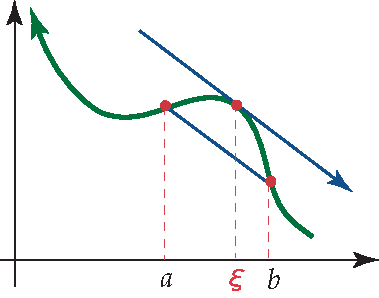
\includegraphics[scale=0.7]{images/ML_fig10}%.pdf
\captionof{figure}{{\small Teorema del valor medio}}
\label{Calculo:fig...}
\end{minipage}
\end{document}